\documentclass{article}
\usepackage[utf8]{inputenc}
\usepackage{amsmath}
\usepackage{systeme,mathtools}
\title{Numerical Mathematics}
\author{Danny Lemmers}
\date{June 2020}

\begin{document}

\maketitle

\section{Numerical and analytical Stability}

To determine the analytical stability of the given system, the first step is to determine the equilibrium or critical points of the system. Using the following system of equations: \\[2ex] $\begin{cases}  ( a-\alpha y_{2}) y_{1} - W(t) y_{1}=0 \\
(-c + \gamma y_{1})y_{2}=0 \end{cases}$ \\[2ex] The first equation can be rewritten as:\\[2ex]
$\begin{array}{lll}
(a- \alpha y_{2}) y_{1} & = & W(t)y_{1}\\
a- \alpha y_{2} & = & W(t)\\
y_{2} & = & \frac{a-W(t)}{ \alpha }
\end{array}$\\[2ex]
Inserting the variables, a = 2, $\alpha = 2 \cdot 10^{-3}$ and $W(t) = 0 \leq W(t) < 2$ gives:\\[2ex]
$\begin{cases}
y_{2} = \frac{2}{2 \cdot 10^{-3}} = 1000 & \mbox{if } W(t) = 0\\
y_{2} = \frac{2-2}{2 \cdot 10^{-3}} = 0 & \mbox {if } W(t) = 2
\end{cases}$\\[2ex]
Rewriting the second equation to find $y_1$ results in:\\[2ex]
$\begin{array}{lll}
-c + \gamma y_{1} = 0\\
y_{1} = \frac{c}{ \gamma }
\end{array}$. Inserting c = 3.92 and $\gamma = 7 \cdot 10^{-3}$ gives: $y_{1} = \frac{3.92}{7 \cdot 10^{-3}} = 560$.\\[2ex]
The next step in determining the stability of a system is to find the eigenvalues of the Jacobi matrix, the Jacobi matrix is defined as: \\[2ex]
$J =\begin{bmatrix}
\frac{\partial u_1}{\partial y_1} &
	\frac{\partial u_1}{\partial y_2} \\[1ex]
\frac{\partial u_2}{\partial y_1} &
	\frac{\partial u_2}{\partial y_2}
\end{bmatrix}$, which in this particular case results in the following matrix:\\[2ex] $ J = \begin{bmatrix}
a-\alpha y_2-W(t) &
    -a y_1 \\[1ex]
\gamma y_2 &
    -c + \gamma y_1
\end{bmatrix}$\newpage
Now to find the eigenvalues for this matrix, determine $\lambda$ in:\\[2ex] $det(J-\lambda I)= 0 =$
$\begin{vmatrix}
a-\alpha y_2-W(t)-\lambda &
    -a y_1 \\[1ex]
\gamma y_2 &
    -c + \gamma y_1 -\lambda
\end{vmatrix}=\\[2ex]\begin{cases}
\begin{vmatrix}
-\lambda &
    -1.12\\
7 &
    -\lambda
\end{vmatrix} &\mbox{if } W(t)=0, \lambda = \pm\sqrt{7.84}i\\[2ex]
\begin{vmatrix}
-\lambda &
    -1.12\\[1ex]
0 &
    -\lambda
\end{vmatrix} &\mbox{if } W(t)=2, \lambda = 0\\
\end{cases}$\\[2ex]
Note that for any W(t) larger than 0, the eigenvalues of the Jacobi matrix is a complex pair, because the lower left part of the matrix becomes a positive value for the defined $\gamma$. \\[2ex]
Now that the eigenvalues are determined, a proper conclusion on both the analytical and numerical stability can be given. For an analytically stable system, the real part of the eigenvalues must be equal or smaller than 0. In this case the eigenvalues are either 0 or purely imaginary, meaning that the real part is always zero, and thus fulfills analytical stability.\\[2ex]
For numerical stability the chosen method is also of importance. In the case of the Runge-kutta 4 method numerical stability is achieved if a sufficiently small time-step $\Delta$t is used. Because the Runge-Kutta method shows stability in the complex plane, the stability can be represented with the following area: \begin{figure}[h]\centering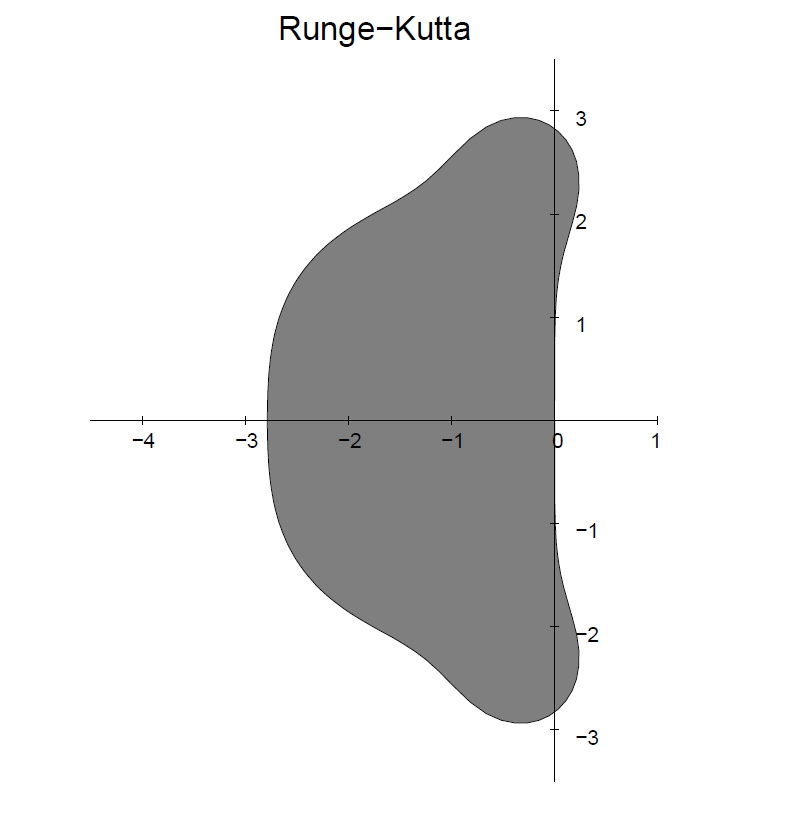
\includegraphics[width=5cm, height = 7cm]{RungeKutta ROC}\caption{Region of Stability for the Runge-Kutta 4 method (C. Vuik et al., 2004)}\label{fig:mesh2}\end{figure} \\As long as $\Delta t \cdot |\lambda_{1,2}(\hat{t},\boldsymbol{\hat{y}})|$ is smaller or equal to 2.8, then the Runge-Kutta 4 method is stable. The size of the time-step is then defined by the formula 
$\Delta t\leq \frac{2.8 }{|\lambda_{1,2}(\hat{t},\boldsymbol{\hat{y}})|}=\frac{2.8}{\sqrt{3.528}}\approx 1.49$. As long as $\Delta t$ is equal to or smaller than 1.49 both analytical and numerical stability is achieved, given this system of equation.



\end{document}
